\chapter{Methodolgy\label{chap:method}}

An important part of any machine learning based detection technique is to choose the most effective machine learning algorithm. For our experiments, we will use various algorithms and try to find the one with the highest accuracy.

\section{Machine Learning}

Machine learning is a field of computer science that helps us automate the process of learning from the data. It helps computers to learn and act without any human intervention~\cite{ML}. The process of learning from the data can be broadly divided into two parts:
\begin{itemize}
	\item Supervised Learning:
	In this the computer is given input data along with the desired outputs and the aim is to learn a function that maps the input data to the desired values.
	\item Unsupervised Learning:
	In this the computer is given only input data without any labels or desired outputs and asked to either predict new data or classify the given input data into separate classes.
\end{itemize}

In our research we labeled the input data as mentioned in Chapter~\ref{chap:dataset} and thus know if a particular connection is malicious or benign. Since we already know the labels of the input data, we use supervised learning algorithms such as Support Vector Machine (SVM), Random Forest, XGBoost and Deep learning based algorithms to train our machine learning models on the input data.

\subsection{Support Vector Machines}

Support Vector Machine (SVM) is a supervised learning algorithm that outputs an optimal separating hyperplane given labeled training data. This hyperplane is then used to classify new samples. The hyperplane is defined by a small subset of the training the training data known as support vectors as shown in Figure~\ref{fig:svm_hyperplane}.

\begin{figure}[htb]
	\centering
	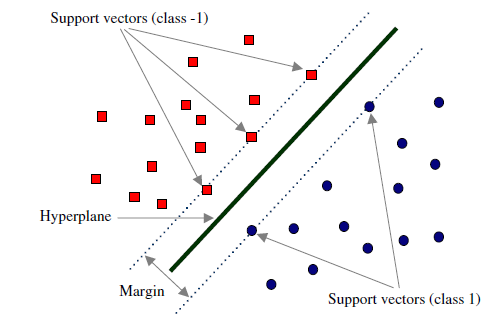
\includegraphics[width=0.7\textwidth]{images/svm-hyperplane.png}
	\caption{SVM hyperplane and support vectors} 
	\label{fig:svm_hyperplane}
\end{figure}

SVM is based on the following three concepts:

\begin{itemize}
	\item Margin Maximization:
	SVM maximizes the margin, i.e. the distance between the support vectors to find the optimal hyperplane as shown in Fig~\ref{fig:svm_hyperplane}
	\item Works in Higher Dimension Space:
	If the training data is not linearly separable, SVM maps the input data to a higher dimensional feature space in which the data is linearly separable as shown in Figure~\ref{fig:svm_kernel}.
	\item Kernel Trick:
	While maximizing the separation margin we do not need the exact points in the higher dimension feature space, but need only their inner products. Getting the inner product is much easier than getting actual points in a higher dimension space. The Kernel trick helps us to operate in a high-dimensional feature space without computing the coordinates of the input data in feature space.
\end{itemize}

One of the advantages of SVM is its effectiveness in high dimensional spaces such as our own data where we have 41 features. Hence, it was a primary choice for our experiments.

\begin{figure}[htb]
	\centering
	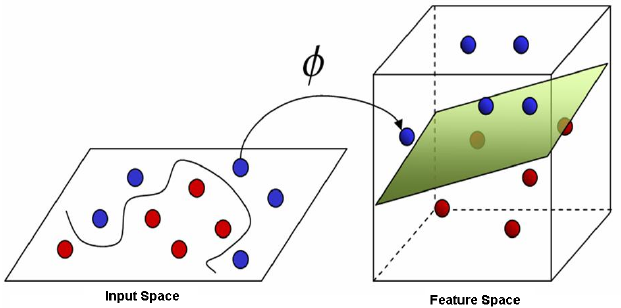
\includegraphics[width=0.5\textwidth]{images/svm-kernel.png}
	\caption{SVM maps input data to feature space} 
	\label{fig:svm_kernel}
\end{figure}

\subsection{Random Forest}

Random Forest is a supervised learning algorithm that is used in classification and regression. It builds an ensemble of decision trees and merges them together to get a stable and more accurate prediction~\cite{Tin95}. As seen in Figure~\ref{fig:random_forest}~\cite{RandomForest}, Random Forest uses bootstrap aggregation also known as bagging to combine predictions from multiple decision trees together to make a more accurate prediction. This reduces the variance of the model without increasing the bias.

\begin{figure}[htb]
	\centering
	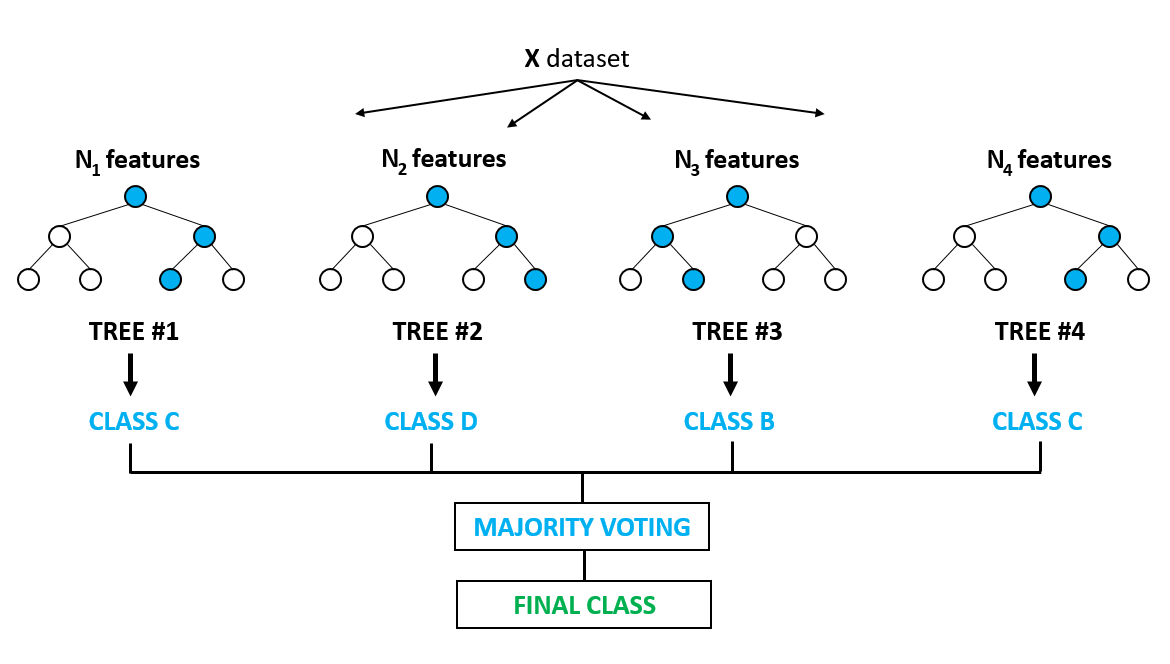
\includegraphics[width=1\textwidth]{images/random_forest.png}
	\caption{Random Forest} 
	\label{fig:random_forest}
\end{figure}

Random Forest is created using the following steps:
\begin{enumerate}
	\item 'K' features are randomly selected from a total of 'm' features such that K<< m
	\item Using the 'K' features a decision tree node is selected using the best split point.
	\item The selected node is further split into child nodes using the best split.
	\item Steps 1-3 are repeared until number of nodes is 1.
	\item Decision tree forest is build by repeating Steps 1-4 for 'n' number of times 
\end{enumerate}

As shown in Figure~\ref{fig:random_forest}, the algorithm follows steps mentioned below to predict the class of the test sample.

\begin{enumerate}
	\item It takes the features of the test sample and goes through each decision tree to predict the outcome.
	\item Calculates the number of votes for each predicted class.
	\item Declares the highest voted class as the final prediction.
\end{enumerate}

\subsection{XGBoost}

XGBoost (eXtreme gradient boosting) is a relatively new software library which was initially started by Tianqi Chen~\cite{ChenG16, XGBWiki} as a research project. It is based upon gradient boosting which is an old machine learning technique used for regression and classification. Like Random Forest, gradient boosting technique also outputs an ensemble of weak decision trees as a prediction model. 

Gradient boosting and Random Forest both use ensemble methods, i.e. building a strong classifier from many weak classifiers. But, the fundamental difference between the two algorithms lies in the methods used to build the strong classifier. Gradient boosting builds on weak classifier sequentially, i.e. one classifier is added at a time which improves upon the already trained ensemble. Whereas in Random Forest bagging is used to create a large number of weak classifiers in parallel, i.e. the classifier is trained independently from the rest.

In mathematical terms, if the ensemble has three trees, the prediction model can be given as
$$
	D(x) = d_{tree 1}(x) + d_{tree 2}(x) + d_{tree 3}(x)
$$
According to gradient boosting the next tree would improve upon the already trained ensemble by minimizes the training error. Thus, the new model $D'(x)$ can then be given as
$$
D'(x) = D(x) + d_{tree 4}(x)
$$

\subsection{Cross-Validation}

Cross-validation is a technique to evaluate how machine learning models perform on a given dataset. It is mainly used in situations such as ours where there is not enough data to divide the dataset into separate training and testing sets. Cross validation can be divided into two types:

\begin{itemize}
	\item Exhaustive cross-validation:
	In this cross-validation method we learn and test on all possible combinations of the training and testing set.
	\begin{itemize}
		\item Leave-\emph{p}-out:
		Leave-\emph{p}-out is a type of exhaustive cross-validation where we use \emph{p} sets as validation set and the remaining are used as training set.
	\end{itemize}
	\item Non-exhaustive cross-validation:
	In this cross-validation method we do not compute all possible combinations of the training and testing set.
	\begin{itemize}
		\item Holdout method:
		This is the simplest cross-validation method where the dataset is separated into two sets, the training and testing set.
		\item \emph{k}-fold cross-validation:
		In this cross-validation method we divide the dataset into \emph{k} subsets and then the model is iteratively tested on one set and trained on the remaining set.
	\end{itemize}
\end{itemize}

We use 10-fold cross-validation in all our experiments. As shown in Figure \ref{fig:10-fold}, our dataset is divided into ten subsets and the model is then iteratively trained on nine subsets and tested on one subset.

\begin{figure}[htb]
	\centering
	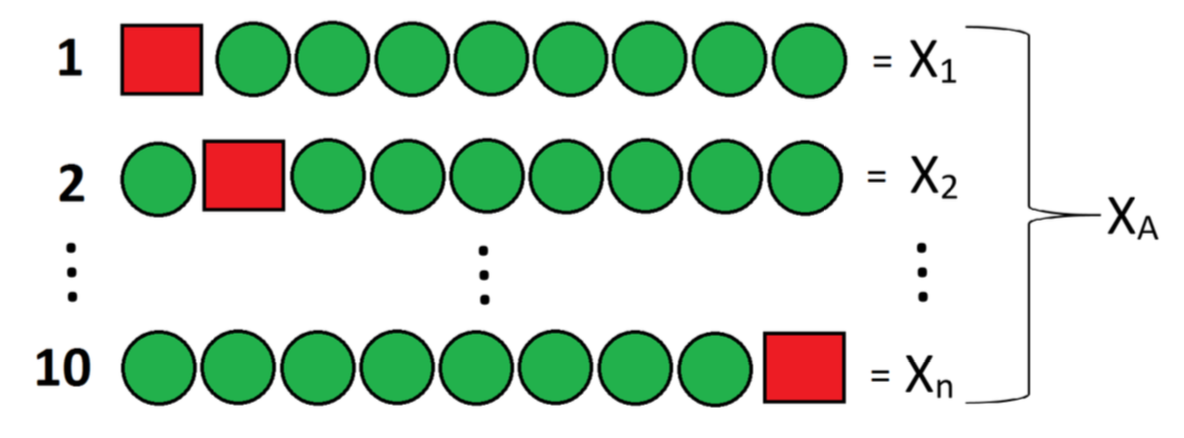
\includegraphics[width=0.7\textwidth]{images/k-fold.png}
	\caption{10-fold cross-validation. The red rectangle is the testing set and the other subsets are used for training.} 
	\label{fig:10-fold}
\end{figure}

\section{Evaluation Metrics}

We use \emph{accuracy} as our evaluation method for all the experiments. \emph{Accuracy} is used to measure how well the model could detect malicious network traffic among the dataset. \emph{Accuracy} can be defined as:
$$
\mbox{Accuracy} = \dfrac{\mbox{TP} + \mbox{TN}}{\mbox{TP} + \mbox{TN} + \mbox{FP} + \mbox{FN}}
$$
where,
\begin{align*}
\mbox{TP: True\;Positives} \\
\mbox{TN: True\;Negatives}\\
\mbox{FP: False\;Positives}\\
\mbox{FN: False\;Negatives}\\
\end{align*}
